\subsection{Gestion de la carte}

Le modele du MVC permet de stocker toutes les données de la simulation. Un carte est un tableau en deux dimensions de taille fixe qui contient des éléments de type Content. Ainsi au démarrage de l'application le modele est initialisé en parsant le fichier de carte sur lequel on veut jouer. Les données lues au moment du parsing sont stockées dans un objet de type Board dont voici la description : \\[0.5cm]
\centerline{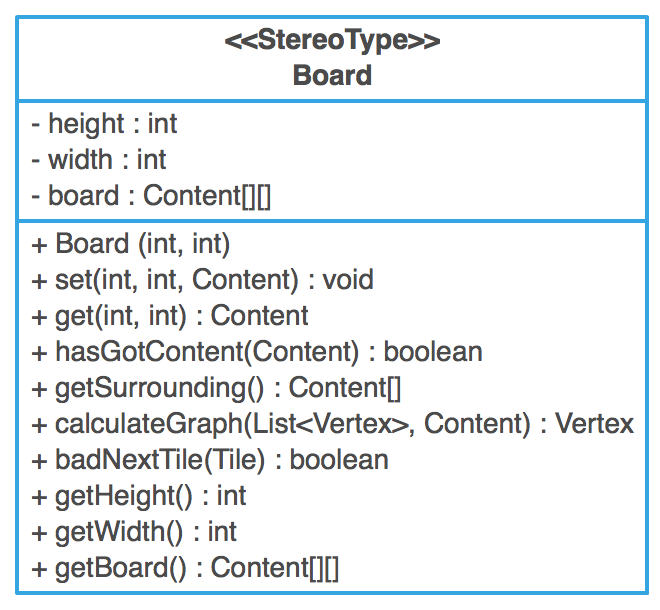
\includegraphics[scale=0.2]{Map}}

Le choix du tableau de taille fixe nous permet d'autre part de gérer les fichiers malformés, les dépassement ce tableau... En effet, c'est grâce à cette objet que nous pouvons tester les cartes "invalides" (les cartes où Pacman ne pourra jamais gagner car il est bloqué).

\subsubsection{vérification de la carte}

Lors du chargement d'une carte une vérification est effectuée afin de déterminer si toutes les pommes de la carte sont accessible par Pacman et si les Fantomes peuvent atteindre Pacman. Pour cela la classe BoardChecker contient une méthode qui va d'abord compter le nombre de cases qui ne sont pas un mur puis sélectionner la première case rencontrée remplissant ces conditions (à condition que la carte ne soit pas composée uniquement de murs). Ensuite l'algorithme visite les cases voisines récursivement jusqu'à avoir visité toutes les cases accessibles par la case d'origine. Le nombre de cases visité est enfin comparée au nombre de cases non-mur total et si ils sont différents, une exception est levée et le programme s'arrête, sinon le jeu peut démarrer.
